\documentclass[11pt]{article}

\usepackage{enumerate}
\usepackage{graphicx}

\title{Efficient Expressions of Probabilistic Programs}
\author{Vlad Firoiu \\ \texttt{vladfi1@mit.edu}}

\begin{document}
\maketitle

\begin{abstract}
Universal probabilistic languages such as Church \cite{Church} can express generative models of arbitrary complexity as functional programs, providing a clear and modular representation of the model. As a tool, the probabilistic language allows models both simple and sophisticiated to be easily written and tested. Inference, often the hardest part of probabilistic modeling in both accuracy and implementation, is done automatically given the program and observed data, usually through approximate MCMC methods. Typically, some random variable in the program is resampled, and the necessary parts of the execution trace are updated accordingly. In this paper, we present methods for writing probabilistic programs so that this inference step is efficient. We shall achieve efficient inference by writing the generative model in a way that allows for parallel execution, thus encoding the conditional independences in the model.
\end{abstract}

\tableofcontents

\section{Operations on Arrays}

A standard construct of imperative programming is looping over an array in order to compute some function of the elements of the array. When the elements of the array are themselves random variables, this introduces a sequential dependency between the partial results computed at each step of the iteration. During inference, if a proposal is made that would modify the value of one of the elements of the array, then this change must propagate through all subsequent iterations, which can be quite inefficient.

Often, this implied dependence is unnecessary. Consider computing the sum of an array of fixed length. Written iteratively, each partial sum depends on the previous partial sum. Conceptually, this corresponds to the following parenthesization of the sum:
\[
(((a_1 + a_2) + a_3) + a_4)
\]
Each sum depends on all internally nested sums. Because addition is associative, we can also write the sum with any parenthesization we choose, such as:
\[
((a_1 + a_2) + (a_3 + a_4))
\]
In this form, it becomes clear that there is no dependence between $(a_1+a_2)$ and $(a_3+a_4)$.

Generalizing to summing over an arbitrary array, we recursively compute the sums of the first and second halves of the array, and then return the sum of these two results. In this form, each variable has only logarithmically many dependent sums. Effectively, we have created a balanced binary tree with the array elements at the leaves, and each each parent the sum of its children.

This operation, which we call \emph{fold}, works with any associative operation, and can easily be written as a recursive procedure:

\begin{figure}[h]
\begin{center}
\begin{verbatim}
[assume fold
    (lambda (op arr min max)
        (let ((avg (int_div (int_plus min max) 2)))
            (if (int_eq min avg)
                (arr min)
                (op
                    (fold op arr min avg)
                    (fold op arr avg max)))))]
\end{verbatim}
\end{center}
\caption{\texttt{fold} in the Venture dialect of Church}
\end{figure}

The execution history of \texttt{fold} exactly mirrors the binary tree, with each recursive call corresponding to a subtree. One can imagine \texttt{fold} executing in parallel by delegating the recursive calls to different processors, resulting in a runtime linear in the height of the tree: $O(\log n)$.

Let us now return to inference. When an element of our array is modified during a Metropolis-Hastings transition, only the ancestors of the corresponding leaf need to be recomputed. Each change to a node in the tree propagates to change in its parent, but not to its sibling. Thus each inference step also takes $O(\log n)$ time. If instead $k$ elements of the array change, then inference over their sum takes $O(k\log n)$ time.

\subsection{Linear Algebra}

One immediate application of \texttt{fold} is to performing basic linear algebra. The dot product of two vectors can easily be written with \texttt{fold}, and this generalizes to arbitrary matrix multiplications. Inference over the product of an $m\times n$ matrix with an $n\times k$ matrix takes $O((m+k)\log n)$ time per transition, assuming that only one matrix entry is reproposed to.

Because matrix multiplication is itself associative, one can use \texttt{fold} to compute the product over an array of matrices, reducing the number of sequential matrix multiplications during inference by a potentially substantial amount. One could imagine this situation arising when doing inference over a complex simulator or dynamical system with many unknown state transitions. In this case, representing the entire model as a probabilistic program could actually speed up inference, at least asymptotically.

\subsection{Range Trees}



\subsection{Limitations}

The first question that might arise is how to do inference over variable length arrays (i.e. non-parametric models). There are two answers to this question. The first relies on the  somewhat arbitrary choice (made by Venture) of reproposing to one random variable in the model uniformly at random. In this case, there is only a $1/n$ chance of resampling the random size of an array of $n$ random variables, and so any linear cost incurred during such a proposal is amortized away.

The second solution requires that there be known some upper bound $N$ on the size of the array. In this case, a \emph{range tree} can be built over all $N$ elements. The range tree computes all of the same partial sums that \texttt{fold} would, enabling it to answer queries for the sum of the elements in some range in $O(\log N)$ time. 

It is also clear that logarithmic inference is not optimal for commutative operations. If only one term of a sum changes, then the new sum can be recomputed in constant time by adding the difference in the modified term to the total. However, it is common for functional algorithms to suffer a logarithmic cost in complexity relative to their procedural analogs. Achieving optimal performance would require additional semantics in the underlying probabilistic language, and is an area of ongoing research.

\section{Sorting}

Another classic problem in algorithms is sorting. The input is again some array of fixed size $n$, and the output is the array in sorted order (or equivalently, the corresponding permutation). While naive algorithms such as insertion sort and selection sort run in $O(n^2)$ time, more sophisticated ones such as mergesort, quicksort, and heapsort can achieve the asymptotically optimal $O(n\log n)$. However, these latter three are inherently sequential: mergesort during the merge step, quicksort during the pivot step, and for heapsort all heap operations. These algorithms can only achieve $O(n)$ in parallel.

The solution is to use a sorting network, such as bitonic sort or odd-even mergesort:

\begin{figure}[h]
\centering
    \includegraphics{bitonic.png}
\caption{Bitonic Sorting Network}
\end{figure}
%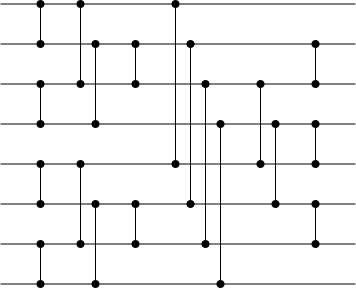
\includegraphics{Batcher_Odd-Even_Mergesort_for_eight_inputs.svg}

These networks can be run in time parallel to their depth, which is $O(\log^2 n)$. There also exist sorting networks of depth $O(\log n)$, but with constant factors that make them useless in practice.

Let us now examine inference over a sorting network. The structure here is much more complicated than the simple binary tree produced by \texttt{fold}; each node (corresponding to a comparison gate) now has two parents instead of one. Unfortunately, this means that a one element change in the input (at depth zero) will result in a two element change at depth one, and the doubling will continue at each layer until every single node is being recomputed. This turns out to be unavoidable. Reproposing one input will result in the shift of some element in the resulting permutation, meaning that possibly linearly many elements of the output must change. This will certainly be the case if the inputs are i.i.d. continuous variables, in which case the reproposed element's new position in the sorted array will be uniform over all $n$ possible positions. Thus inference over any sorting algorithm can do no better than $\Omega(n)$, which is not much better than the $\tilde{O}(n)$ achieved by forward simulation. It may still be possible, however, to sort arrays which from the prior are nearly sorted, or whose transition kernels guarantee only small perturbations to the output. 

\subsection{Permutations}

Though sorting may not be amenable to inference, parallel sorting networks turn out to still be useful for writing probabilistic programs. Suppose that instead of comparison gates, the sorting network was equipped with noisy swap gates, which with probability $1/2$ swap their inputs and with probability $1/2$ do nothing. Essentially, each gate independently applies a random permutation to its two inputs.

\begin{thebibliography}{9}
\bibitem{Church}
    Noah D. Goodman, Vikash K. Mansinghka, Daniel M. Roy, Keith Bonawitz, and Joshua B. Tenenbaum. Church: a language for generative models. \emph{Uncertainty in Artificial Intelligence} \textbf{24} 220-229 (2008)
\end{thebibliography}

\end{document}
